%%%%%%%%%%%%%%%%%%%%%%%%%%%%%%%%%%%%%%%%%
% Arsclassica Article
% LaTeX Template
% Version 1.1 (10/6/14)
%
% This template has been downloaded from:
% http://www.LaTeXTemplates.com
%
% Original author:
% Lorenzo Pantieri (http://www.lorenzopantieri.net) with extensive modifications by:
% Vel (vel@latextemplates.com)
%
% License:
% CC BY-NC-SA 3.0 (http://creativecommons.org/licenses/by-nc-sa/3.0/)
%
%%%%%%%%%%%%%%%%%%%%%%%%%%%%%%%%%%%%%%%%%

%----------------------------------------------------------------------------------------
%	PACKAGES AND OTHER DOCUMENT CONFIGURATIONS
%----------------------------------------------------------------------------------------

\documentclass[
10pt, % Main document font size
letterpaper, % Paper type, use 'letterpaper' for US Letter paper
oneside, % One page layout (no page indentation)
%twoside, % Two page layout (page indentation for binding and different headers)
headinclude,footinclude, % Extra spacing for the header and footer
english
]{article}

%%%%%%%%%%%%%%%%%%%%%%%%%%%%%%%%%%%%%%%%%
% Arsclassica Article
% Structure Specification File
%
% This file has been downloaded from:
% http://www.LaTeXTemplates.com
%
% Original author:
% Lorenzo Pantieri (http://www.lorenzopantieri.net) with extensive modifications by:
% Vel (vel@latextemplates.com)
%
% License:
% CC BY-NC-SA 3.0 (http://creativecommons.org/licenses/by-nc-sa/3.0/)
%
%%%%%%%%%%%%%%%%%%%%%%%%%%%%%%%%%%%%%%%%%

%----------------------------------------------------------------------------------------
%	REQUIRED PACKAGES
%----------------------------------------------------------------------------------------

\usepackage[
nochapters, % Turn off chapters since this is an article        
beramono, % Use the Bera Mono font for monospaced text (\texttt)
eulermath,% Use the Euler font for mathematics
pdfspacing, % Makes use of pdftex’ letter spacing capabilities via the microtype package
dottedtoc % Dotted lines leading to the page numbers in the table of contents
]{classicthesis} % The layout is based on the Classic Thesis style

\usepackage{arsclassica} % Modifies the Classic Thesis package

\usepackage[T1]{fontenc} % Use 8-bit encoding that has 256 glyphs

\usepackage[utf8]{inputenc} % Required for including letters with accents

\usepackage{graphicx} % Required for including images
\graphicspath{{Figures/}} % Set the default folder for images

\usepackage{enumitem} % Required for manipulating the whitespace between and within lists

\usepackage{lipsum} % Used for inserting dummy 'Lorem ipsum' text into the template

\usepackage{subfig} % Required for creating figures with multiple parts (subfigures)

\usepackage{amsmath,amssymb,amsthm} % For including math equations, theorems, symbols, etc

\usepackage{varioref} % More descriptive referencing

%----------------------------------------------------------------------------------------
%	THEOREM STYLES
%---------------------------------------------------------------------------------------

\theoremstyle{definition} % Define theorem styles here based on the definition style (used for definitions and examples)
\newtheorem{definition}{Definition}

\theoremstyle{plain} % Define theorem styles here based on the plain style (used for theorems, lemmas, propositions)
\newtheorem{theorem}{Theorem}

\theoremstyle{remark} % Define theorem styles here based on the remark style (used for remarks and notes)

%----------------------------------------------------------------------------------------
%	HYPERLINKS
%---------------------------------------------------------------------------------------

\hypersetup{
%draft, % Uncomment to remove all links (useful for printing in black and white)
colorlinks=true, breaklinks=true, bookmarks=true,bookmarksnumbered,
urlcolor=webbrown, linkcolor=RoyalBlue, citecolor=webgreen, % Link colors
pdftitle={}, % PDF title
pdfauthor={\textcopyright}, % PDF Author
pdfsubject={}, % PDF Subject
pdfkeywords={}, % PDF Keywords
pdfcreator={pdfLaTeX}, % PDF Creator
pdfproducer={LaTeX with hyperref and ClassicThesis} % PDF producer
} % Include the structure.tex file which specified the document structure and layout
\usepackage[letterpaper]{geometry}
\geometry{verbose,tmargin=1in,bmargin=1.5in,lmargin=1.5in,rmargin=1.5in}

\hyphenation{Fortran hy-phen-ation} % Specify custom hyphenation points in words with dashes where you would like hyphenation to occur, or alternatively, don't put any dashes in a word to stop hyphenation altogether

%----------------------------------------------------------------------------------------
%	TITLE AND AUTHOR(S)
%----------------------------------------------------------------------------------------

\title{\normalfont\spacedallcaps{CIS 559 Project 1:\break Parallel Football}} % The article title

\author{\spacedlowsmallcaps{Ian Sibner, Derick Olson, Spriha Baruah, Anthony Hsieh}} % The article author(s) - author affiliations need to be specified in the AUTHOR AFFILIATIONS block

\date{22 September 2015} % An optional date to appear under the author(s)

%----------------------------------------------------------------------------------------
\setlength\parindent{0pt}
\setlength{\parskip}{1em}

\begin{document}

%----------------------------------------------------------------------------------------
%	HEADERS
%----------------------------------------------------------------------------------------

\renewcommand{\sectionmark}[1]{\markright{\spacedlowsmallcaps{#1}}} % The header for all pages (oneside) or for even pages (twoside)
%\renewcommand{\subsectionmark}[1]{\markright{\thesubsection~#1}} % Uncomment when using the twoside option - this modifies the header on odd pages
\lehead{\mbox{\llap{\small\thepage\kern1em\color{halfgray} \vline}\color{halfgray}\hspace{0.5em}\rightmark\hfil}} % The header style

\pagestyle{scrheadings} % Enable the headers specified in this block

%----------------------------------------------------------------------------------------
%	TABLE OF CONTENTS & LISTS OF FIGURES AND TABLES
%----------------------------------------------------------------------------------------

\maketitle % Print the title/author/date block

\setcounter{tocdepth}{2} % Set the depth of the table of contents to show sections and subsections only

\tableofcontents % Print the table of contents

\listoffigures % Print the list of figures

% \listoftables % Print the list of tables

%----------------------------------------------------------------------------------------
%	ABSTRACT
%----------------------------------------------------------------------------------------

\section{Introduction} % This section will not appear in the table of contents due to the star (\section*)

Parallel Soccer is a game in which four teams of $P$ (which can vary from 1 to 250) players compete to kick soccer balls into their teams' goal. The goals are arranged in each corner of a 32x32 grid, and the rest of the squares on the board are initialized to contain one ball each, for a total of $1,020$ balls on the board to start off with. To start off with, each team can place each of their $P$ players anywhere on the board; multiple players can potentially occupy the same square. After that, each player (with full knowledge of the board) must choose to either \textit{kick} a ball (in their square) up to $K$ distance away (with $K$ being a constant whose value may vary between one and 45), or \textit{move} up to 1 square in any direction (including diagonals). When a ball is kicked into a team's goal, that team is awarded a point and the ball is removed from play. The game ends when all balls are removed from play, and the team with the most points wins.

\begin{figure}[tb]
\centering 
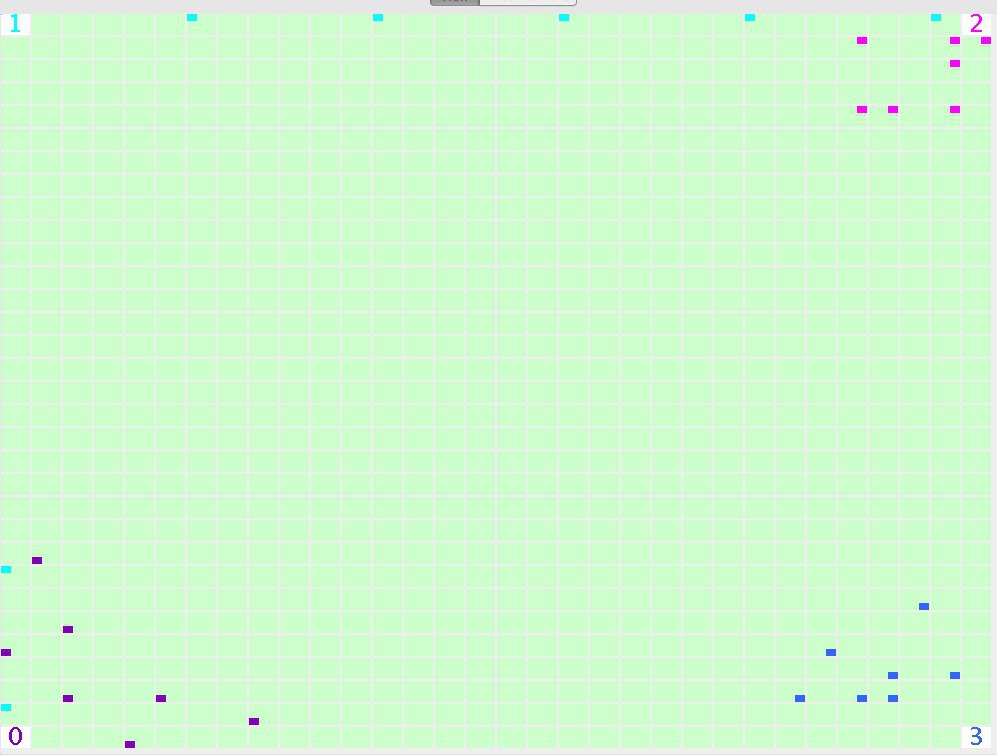
\includegraphics[width=0.8\columnwidth]{initial-position} 
\caption[Initial board of a parallel football game]{An initial positioning of the board where $P=7$}
\label{fig:gallery} 
\end{figure}

\section{Initial Insights and Observations}

Immediately, our team observed several key features about the game. 

\begin{enumerate}
  \item The game is zero-sum. That is, any ball that is scored by our player is denied to all of our opponents, and vice versa.
  \item Efficiency is not a constraint. Because the game would not progress to the next step until all of our players had calculated their next move, we could take the entire board into account without worrying about the runtime of our solution.
  \item Strategies may work well for certain combinations of $P$ and $K$ and not others. A smart player would change its strategy depending on what value these constants took on.
  \item Certain strategies may work particularly well in the early phase of the game, when all the balls are on the board and there are not clusters, while others may work better in the middle phase (where there are fewer balls and more clusters) or in the end game (when there are only a few balls which every team is competing for).
  \item Efficient strategies (i.e. those which required to fewest moves to kick a ball into the goal) would generally favor kicking over moving, since $K \geq 1$. This naturally leads to a sort of ``bucket brigade'' where players kick balls close to one another in order to ``pass'' them towards the goal.
\end{enumerate}

These insights guided our strategy throughout and allowed us to focus on the most important aspects of the game.

\section{Strategies and Concepts}

\subsection {Movement \& Benefit Function}

In order for a player to decide which cell was the best move for any given board state, we created a benefit function that assigned a score to each cell for every given player. Since we had access to the entire board, we used many factors in this function, including the number of balls in a cell (and surrounding cells), distance from the cell to our goal, distance from the cell to the player, and the number of opponents around the cell. Given the loose efficiency constraints given the problem, we decided that a globally optimal benefit function would be both feasible and desirable. The primary gain from this decision was a team optimized for late gameplay, where our players were able to seek out and steal balls toward the end of the game. The reason was that once we and other teams cleared the balls near our respective goals, balls became scarce. If any team had accumulated balls, even if they were far from our players, they would seek them out and attempt to score with them.

On the other hand, as teams improved, the game time grew shorter and quicker. In such a game, it is possible that a globally optimal zone will change into a depleted zone before a far-away team can reach it. It is likely that our model did not fully capture the constantly changing state of the game board. We addressed this by heavily weighting our own goal in benefit calculations.

\subsection{Cell clustering}
On the second iteration of our benefit function, we accounted for ball and opponent clustering by keeping track of the number of balls and opponents surrounding a particular cell. This allowed our players to seek out areas of high benefit, rather than single cells. 

After initial trials with a large radius, we settled on a radius of 3. We observed that larger radii caused the players to move back and forth somewhat inefficiently, and hypothesize that these larger zones changed too quickly for players to capitalize on them.


\section{Implementation}

\subsection{Composability}
Because we realized that certain strategies might work very well in the early phase while others might excel in the late phase, we set about building a player that would \textit{compose} other players by switching between its component players' strategies. We met with a lot of success the first week by composing Group 1's \texttt{GridPlayer} for the first 200 turns and our own mid-game-optimized \texttt{DerickPlayer} for the remainder of the game. This worked about as expected; \texttt{GridPlayer} was far more efficient than \texttt{DerickPlayer} in the early game, but after about 200 turns, the board had grown sparser and our own player was much better at seeking out balls and scoring them. We believed this was the way forward and set about finding a more intelligent way to determine when to switch (factoring in $P$, $K$, and the number of balls left on the board).

However, during the third week of gameplay, the rest of the teams (and our own \texttt{DerickBrigadePlayer}) had become so sophisticated that the early stage of the game completely dominated. Essentially, the winner was determined by how well the early phase played out, and the middle/end phases were nearly nonexistent. Thus we decided to play a pure strategy in the final round, focused on early-game optimization, rather than continuing to compose multiple strategies.

\begin{figure}[tb]
\centering 
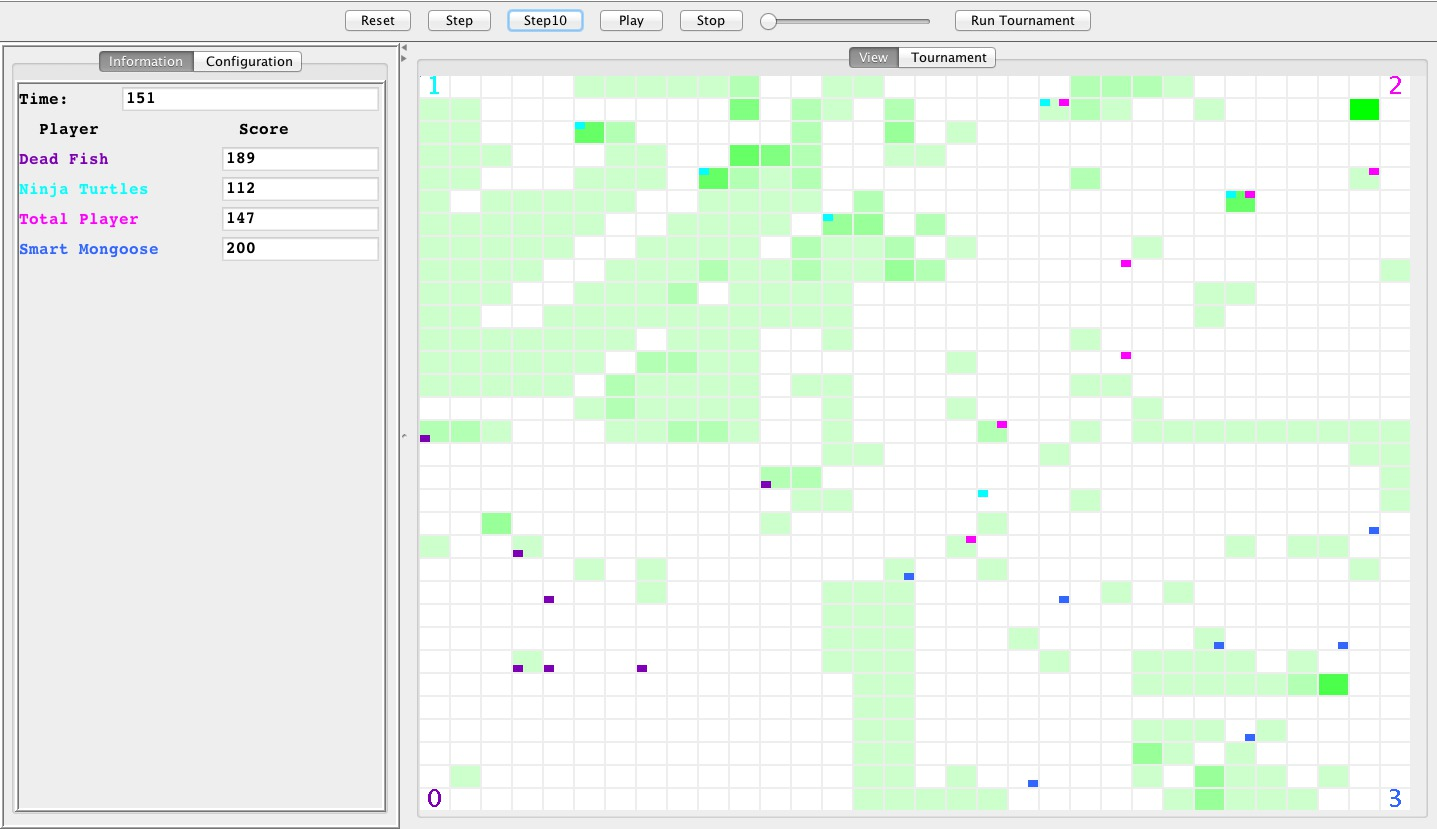
\includegraphics[width=0.8\columnwidth]{after150} 
\caption[State of a parallel football board after 150 turns]{The state of the board after 150 turns with $P=7$, $K=6$. Note how over 60\% of the balls are already scored; this illustrates the great importance of the early game when sophisticated strategies are placed in competition.}
\label{fig:gallery} 
\end{figure}

\section{Results}

\lipsum[3]

\section{Contributions}

\lipsum[2]

\section{Future Directions and Limitations}

\subsection{Strengthen Early Game Through Sweeping}
Among teams that placed highly in the tournament, we noticed that their players would tend to start the game by sweeping balls inwards towards their own goal, maximizing their early-game wins before beginning to spread out across the board. Our players, which started close to our own goal, did not exhibit this behavior. Adapting our placement strategy so that they started farther away might be sufficient to achieve this result; however, we could also look into a composability solution in which a sweeping strategy is used for the very first portion of the game before switching to our current players' behavior. This would require significantly tweaking our composability behavior, particularly the point at which the behavior switch occurred, in order to ensure that our players did not continue sweeping for too long before switching to mid-game behavior.

\subsection{Generalized Step Distance}
This idea stems from our attempts to take advantage of global-scope “hotspots,” or high-density ball clusters that are not near the goal. The existing implementation weights balls close to the home goal particularly high, which is good in the early game, but may not be ideal overall. 

As we can see in the figure above, certain strategies tend to cluster balls near an opponent goal, where they stay relatively untouched for several cycles. A smarter global-cluster detection would drop the current strategy 

The biggest disadvantage to this approach is that the time it takes to travel to such a cluster may be greater than the the time the cluster exists. Even if the seeking team is able to reach the cluster in time, the balls lost in the transit time may not be worth it.

It would be possible to determine, by factoring in the number of balls left $B_{total}$, the number of balls in close range $B_{nearby}$, and the number of balls expected to remain in the cluster $B_{cluster}$. Such a strategy would decide to go for the cluster if and only if: 
$$B_{total} - B_{nearby} < B_{cluster}$$

One way of implementing this strategy would be to generalize the  \texttt{numberOfStepsToGoal()} benefit function to be \texttt{numberOfStepsToPosition(p)}, where the latter takes in any valid position $p$ as it’s argument, causing the cells around it to get a score boost. Then, upon deciding to pursue a cluster, this position would be updated to the cluster center, until a new position was found.

\section{Acknowledgments}

Our progress was largely a result of the class discussions and adopted strategies. Through the course of the project, we adopted starting strategies from Groups 1 (Grid Player), as well as experiments in stealing opponent balls with the opening placements. We would like to give special thanks to Groups 2 and 6 for the important heuristics we adopted from them and eventually used in our final implementation. 

Group 2 (The Swarm) was the first group to successfully implement a kind of benefit function with the emergent behavior of a bucket brigade. This function was based on the number of steps from the ball to the goal, and we adopted it as a core feature of our ensemble benefit function.

Group 6 (Bucket Brigade) contributed a smarter kicking function that favored passing to players over kicking as far to the goal as possible. We adopted this function as a core part of our improved kicking strategy.

\section{Conclusion}

\lipsum[1]

\end{document}
